% !TEX TS-program = pdflatexmk
\documentclass[11pt,a4paper]{article}

\usepackage[english]{babel}
\usepackage[T1]{fontenc}
\usepackage{graphicx}
\usepackage{indentfirst}
\usepackage[applemac]{inputenc}
\usepackage{url}

\begin{document}

\thispagestyle{empty}

\begin{center}
{\huge Politecnico di Milano}
\end{center}

\begin{center}
{\huge Argomenti Avanzati di Ingegneria del Software}
\end{center}

\vskip 8cm

\begin{center}
{\huge An adaptive cache server written in F\#}\\
\url{http://code.google.com/p/adaptive-cache-server/}
\end{center}

\vskip 2cm

\begin{center}
\begin{tabular}{ll}
{\large Filippo Sironi} & {\large 734456}\\
{\large Matteo Villa} & {\large 735064}\\
\end{tabular}
\end{center}

\vskip 2cm

\begin{center}
{\large 2009-2010}
\end{center}

\newpage

\section{Introduction}
\label{section:introduction}
Aim of this project is to explore the support that a given programming language and, if available, the underlying framework can provide in order to build an aware and adaptive software system.
While adaptation can be achieved through primitive constructs (such as an \textit{if} or \textit{case} chain that selects the desired behavior), our goal is to rely on a more powerful level of abstraction and higher level constructs among the ones offered by the platform.

The programming language adopted for this project is F\#, a multi-paradigm programming language leveraging the .NET framework.

\section{The F\# programming language and the .NET framework}
\label{section:platform}
The F\# project began in 2002 when Don Syme and others at Microsoft Research decided to propose the adoption of a functional programming language based on \textit{ML} for the .NET framework. Its first major pre-release was in 2005.

F\# is a statically strong typed programming language that supports many different paradigms. It shares a core language with the OCaml (Objective Caml) programming language, and in some ways it can be considered an ``OCaml for .NET''. F\# would not exist without OCaml, which in turn comes from the ML family of programming languages, which dates back to 1974. F\# also draws from the Haskell programming languages and other functional programming languages such as Erlang.

Despite being a functional programming language and being similar to OCaml and Haskell, we can say that F\# is a whole other kind of programming language. In fact, F\# can leverage the full power of .NET that allows the natural adoption of both the imperative and the object-oriented (OO) paradigms; moreover, F\# allows the exploitation of advanced constructs such as sequence expressions and workflows which are inspired by Haskell's monads. In addition to this, F\# also provides a missing link between compiled and the so called dynamic programming languages, combining the idioms and programming styles typical of dynamic programming languages with the performance and robustness of a compiled programming language.

Functional programming is booming at a point that some common functional programming constructs have been integrated into mainstream programming languages such as C\#, Python, Ruby, and more recently, Java.

\section{An adaptive cache server written in F\#}
\label{section:work}
The software system to build for this project is a cache server. As a basic behavior it simply offers a caching service, speeding up the retrieval of information generated on other machines. The type of items to store in the cache can be resources of any kind. The server exposes some simple primitives, such as \texttt{search(key)}, \texttt{store(value)}, and \texttt{remove(key)}. The cache server must be aware and adaptive.

The cache server implemented for this project leverages awareness and adaption in different contexts. In fact, it provides adaptation in accordance with the memory context, the logging context, and the network context.

\subsection{Memory context}
\label{section:work:memory-context}
The implemented cache server supports theoretically an infinite number of memory contexts which are partition in two major contexts. The first is called \textit{high memory context} while the second is \textit{low memory context}.

When the \textit{high memory context} is active the cache server is allowed to use an infinite amount of virtual memory and the sole memory limitation is given by the total amount of virtual memory the machine can address. This means every cache line is ``volatile'' in the sense that it is only resident within the volatile memory.

On the other hand, when the \textit{low memory context} is active there can be many different situations. The low memory context is coupled with a parameter indicating the upper bound of volatile memory the cache server can use to store cache lines. Once the bound is reached the cache server starts using the non-volatile memory.

\subsection{Logging context}
\label{section:work:logging-context}
Many different software systems support many different levels of logging. Usually the logging level is selected when the software system is started and cannot be changed at run-time. A peculiarity of aware and adaptive software systems is the capability of changing the way they operate without any down-time: therefore, the cache server here implemented has indeed the ability to change the amount of messages to be logged during its execution. It supports three different logging levels:
\begin{description}
\item [\textit{Error}:] only error messages are logged;
\item [\textit{Warning}:] warning and error messages are logged;
\item [\textit{Information}:] (verbose context) logs information, warning, and error messages.
\end{description}

\subsection{Network context}
\label{section:work:network-context}
The last adaptation capability implemented is that regarding the network context. The cache server supports the ability to change the protocol used for the client/server communication while the system is running without any interruption.

\subsection{Implementation}
\label{section:work:implementation}
The cache server is logically partitioned in five different modules, as shown in Figure \ref{figure:modules}.

\begin{figure}
\begin{center}
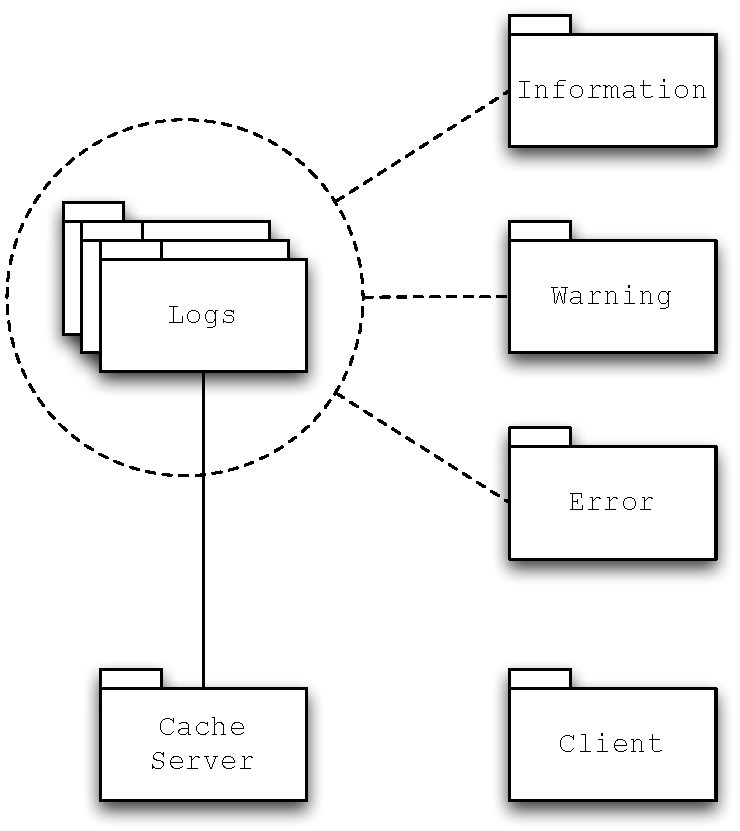
\includegraphics[width=0.75\textwidth]{figures/Modules.pdf}
\caption{Modules}
\label{figure:modules}
\end{center}
\end{figure}

The \textit{client} module contains all the code related to the client used to interact with the cache server; the \textit{cache server} module contains the code related to the server itself; while the three modules \textit{error}, \textit{warning}, and \textit{information} contain the code used to handled the three logging levels. Further explanations about this partitioning will be given later.

The client is a simple interactive application that has been developed making an extensive use of the functional programming paradigm. The mutable state is concentrated in a set of mutable values which are used to handle the hot-swap of a network protocol, hence the change of the network context, in favor of another one. The application' s configuration is read, once the application is started, from an XML configuration file.

The cache server is composed of different elements organized in different sub-modules, as Figure \ref{figure:server-modules} shows.

\begin{figure}
\begin{center}
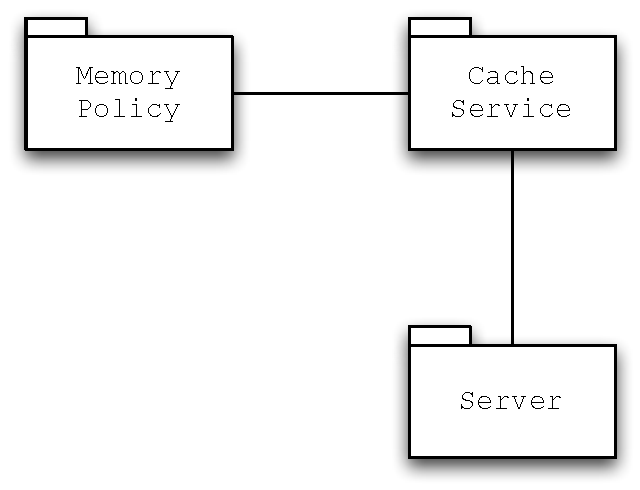
\includegraphics[width=0.65\textwidth]{figures/Server-Modules.pdf}
\caption{Modules}
\label{figure:server-modules}
\end{center}
\end{figure}

The \textit{server} module contains an interactive application whose execution cycle is split in two asynchronous tasks (threads). One of the task maintains an instance to the cache service (implemented by the \textit{cache service} module) while the other handles network communications and accesses the cache service running within the other task. Finally, the \textit{memory policy} module contains the code that handles the different memory contexts. Just like the client, the cache server loads its initial configuration from an XML file.

\section{Involved abstractions and constructs}
\label{section:functionalities}

\section{Conclusions}
\label{section:conclusions}

\end{document}
